%%%%% Description: history of (weak) consistency models in the context of distributed systems. %%%%%
%%%%% Date: July 14, 2016 %%%%%
%%%%% Author: Hengfeng Wei %%%%

\documentclass{standalone}

\usepackage{tikz}
\usetikzlibrary{positioning, shapes, shapes.symbols, backgrounds, fit, arrows.meta, calc}
\usepackage{varwidth}

\begin{document}
\begin{tikzpicture}[comment/.style = {align = center}]
  %%%%%%%%%% Begin: years and papers %%%%%%%%%% 
  % \x: x coordinate; \y: year; \n: name; \lbl: label
  \foreach \x/\y/\n/\lbl in {
  	1/1995/eventual/eventual consistency, 
	6/2000/cap/CAP theorem,
	11/2006/bigtable/Bigtable@Google,
    15/2007/dynamo/Dynamo@Amazon, 
    20/2012/pacelc/PACELC tradeoff} {
	\node[star, star points = 5, minimum size = 3pt, draw = red, fill = yellow, line width = 2pt] (\x) at (\x, 5) {};
	\node[below = 0.50cm of \x] (\y) {$\y$};
	\node[above = 0.50cm of \x, align = center] (\n) {\lbl};
  }

  \path[draw = red, dashed, very thick] (1) to (6) to (11) to (15) to (20);
  \draw[-latex, draw = red, dashed, very thick] (20) to (22, 5);
  %%%%%%%%%% End: decades and systems %%%%%%%%%% 

  %%%%% bayou system %%%%%
  \node[below = of 1995] (bayou-fig) {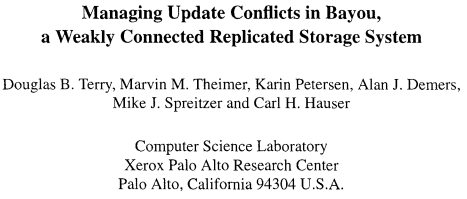
\includegraphics[scale = 0.35]{figs/bayou-paper.png}};
  \node[above = of eventual] (bayou-eventual) {
\includegraphics[scale = 0.09]{figs/available-checked.png}};

  %%%%% cap theorem %%%%%
  \node[below = of 2000] (cap-ppt) {
\includegraphics[scale = 0.35]{figs/cap-keynote-ppt.png}};
  \node[above = of cap] (cap-fig) {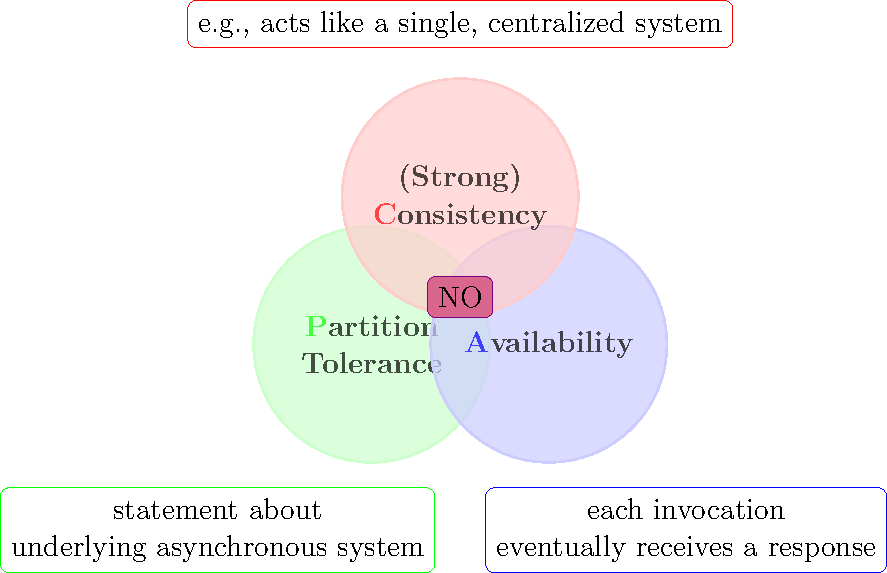
\includegraphics[scale = 0.35]{figs/cap-theorem.pdf}}; 

  %%%%% bigtable %%%%%
  \node[below = of 2006] (bigtable-fig) {
\includegraphics[scale = 0.45]{figs/google-bigtable-text.jpg}};
  \node[above = of bigtable] (bigtable-tradeoff) {
\includegraphics[scale = 0.08]{figs/unavailable.png}};

  %%%%% dynamo %%%%%
  \node[below = of 2007] (dynamo-fig) {
\includegraphics[scale = 0.35]{figs/dynamo-logo.jpg}};
  \node[above = of dynamo] (dynamo-tradeoff) {
\includegraphics[scale = 0.05]{figs/eventually.jpg}};  % with the 24-7-365 image

  %%%%% more systems %%%%%

  %%%%% pacelc tradeoff %%%%%
  \node[below = of 2012] (pacelc-paper) {
\includegraphics[scale = 0.10]{figs/ieee-computer12-front-cover.pdf}};
  \node[above = of pacelc] (pacelc-fig) {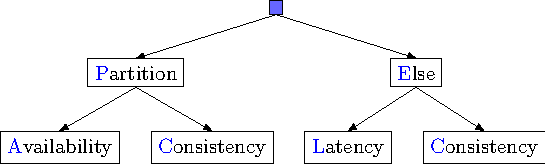
\includegraphics[scale = 0.60]{figs/pacelc-tradeoff.pdf}};
  %%%%% %%%%%
  %%%%% %%%%%
\end{tikzpicture}
\end{document}
